\setchapterpreamble[u]{\margintoc}
\chapter{Answers}
\labch{ch-answers}


Tasks and questions are scattered throughout the book, 
and the answers are collected in this chapter.


\section{Introduction}
\labsec{answer-intro}


\begin{exercise}%
    \label{answer:short-link-to-SPARQL}
How to create a short link to a SPARQL script?
\end{exercise}

\begin{marginfigure}[0cm]
    {%
        \setlength{\fboxsep}{0pt}
        \setlength{\fboxrule}{1pt}
        \fcolorbox{gray}{gray}{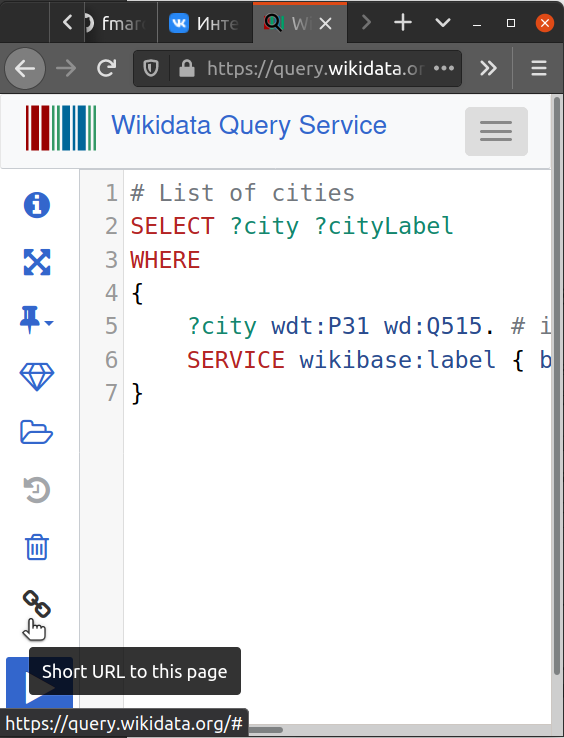
\includegraphics[width=\linewidth]{chapter/intro/WD_Query_Service_Short_URL_2020.png}}
    }
	\caption{The chain symbol button creates a short link to the SPARQL script, Wikidata Query Service, 2020.}
	\labfig{fig:WDQS-Short-URL-creation}
\end{marginfigure}

The Wikidata Query Service is shown in~\reffig{fig:WDQS-Short-URL-creation}. 
The bottom button with a chain symbol allows you to create a short link to the SPARQL script. 

See question on page~\pageref{question:short-link-to-SPARQL}.



\section{Aircraft from small to large}
\labsec{answer-aircraft}

%%%%%%%%%%%%%%%%%%%%%%%%%%%%answer_1%%%%%%%%%%%%%%%%%%%%%%

\begin{exercise}%
    \label{answer:aircraft_manufacturers_en}
Which Russian aircraft manufacturers have websites?
\begin{itemize}
\item MiG
\item Saratov Aviation Plant
\item Tupolev
\item Sukhoi
\end{itemize}
\end{exercise}

The following Russian manufacturers have websites: Mig, Tupolev and Sukhoi. The answer to the question can also be obtained by running the following SPARQL query (listing~\ref{lst:aircraft_listing_Manufacturers_websites}). 
    
\begin{lstlisting}[ language=SPARQL, breaklines=true, 
                    caption={Manufacturers websites\\\hspace{\textwidth}
                        SPARQL query: \href{https://w.wiki/rg8}{w.wiki/rg8}
                        },
                    label=lst:aircraft_listing_Manufacturers_websites,
                    texcl 
                    ]
SELECT ?manufacturer ?manufacturerLabel ?site
WHERE
{
    ?manufacturer wdt:P31 wd:Q936518. # instance of aerospace manufacturer
  	?manufacturer wdt:P17 wd:Q159. # country Russia
  	?manufacturer wdt:P856 ?site # official website
    SERVICE wikibase:label { bd:serviceParam wikibase:language "en" }
}
\end{lstlisting}

Question from page~\pageref{question:aircraft_manufacturers_en}.

%%%%%%%%%%%%%%%%%%%%%%%%%%%%answer_2%%%%%%%%%%%%%%%%%%%%%%

\begin{exercise}%
    \label{answer:aircraft_answer_2}
Find the correspondence between the date of foundation and the company.
\\
\begin{tabular}{ l | l }
Company & Foundation date \\ \hline
MiG & 01.01.1939 \\
Vympel & 18.11.1949 \\
Tupolev & 18.12.1939 \\
Sukhoi & 01.01.1922 \\
\end{tabular}
\end{exercise}

The company ``Mig" was founded on December 18.1939, ``Pennant" - November 18.1949, ``Tupolev" - January 01.1922, ``Sukhoi" - January 01.1939 Reply the question can also be obtained by running the following SPARQL-request (listing \ref{lst:aircraft_company_foundation_date_lst_en}). 
       
\begin{lstlisting}[ language=SPARQL, breaklines=true, 
                    caption={Company foundation dates\\\hspace{\textwidth}
                        SPARQL query: \href{https://w.wiki/rg7}{w.wiki/rg7}
                        },
                    label=lst:aircraft_company_foundation_date_lst_en,
                    texcl 
                    ]
SELECT ?manufacturer ?manufacturerLabel ?inception
WHERE
{
    ?manufacturer wdt:P31 wd:Q936518. # instance of aerospace manufacturer
  	?manufacturer wdt:P17 wd:Q159. # country Russia
  	?manufacturer wdt:P571 ?inception # foundation date
    SERVICE wikibase:label { bd:serviceParam wikibase:language "en" }
}
\end{lstlisting}

Question from page~\pageref{question:aircraft_question_2}.

%%%%%%%%%%%%%%%%%%%%%%%%%%%%answer_3%%%%%%%%%%%%%%%%%%%%%%

\begin{exercise}%
    \label{answer:aircraft_company_headquarters_en}
Find the correspondence between the location of the company's headquarters and the company.
\\
\begin{tabular}{ l | l }
Company & Headquarters \\ \hline
Kazan Helicopters Plant & Kazan \\
Saratov Aviation Plant & Saratov \\
Ulan-Ude Aviation Plant & Ulan-Ude \\
Sukhoi & Moscow \\
\end{tabular}
\end{exercise}

The headquarters of the company ``Kamov" is located in the city of Lyubertsy, ``Aviadvigatel" - the city of Perm, ``Ulan-Ude Aviation Plant" - the city of Ulan-Ude, ``Sukhoi" - the city of Moscow. The answer to the question can also be obtained by running the following SPARQL-request (listing \ref{lst:aircraft_company_headquarters_lst_en}). 
          
\begin{lstlisting}[ language=SPARQL, breaklines=true, 
                    caption={Company headquarters\\\hspace{\textwidth}
                        SPARQL query: \href{https://w.wiki/rg5}{w.wiki/rg5}
                        },
                    label=lst:aircraft_company_headquarters_lst_en,
                    texcl 
                    ]
SELECT ?manufacturer ?manufacturerLabel ?inceptionLabel
WHERE
{
    ?manufacturer wdt:P31 wd:Q936518. # instance of aerospace manufacturer
  	?manufacturer wdt:P17 wd:Q159. # country Russia
  	?manufacturer wdt:P159 ?inception # headquarters location
    SERVICE wikibase:label { bd:serviceParam wikibase:language "en" }
}
\end{lstlisting}

Question from page~\pageref{question:aircraft_question_3}.

%%%%%%%%%%%%%%%%%%%%%%%%%%%%answer_4%%%%%%%%%%%%%%%%%%%%%%

\begin{exercise}%
    \label{answer:aircraft_question_airship_en}
What is the name of the aircraft, supported in flight by a huge cylinder of flammable, lethal gas, right above the heads of the passengers?
\end{exercise}

\begin{marginfigure}[0cm]
    {%
        \setlength{\fboxsep}{0pt}
        \setlength{\fboxrule}{1pt}
        \fcolorbox{gray}{gray}{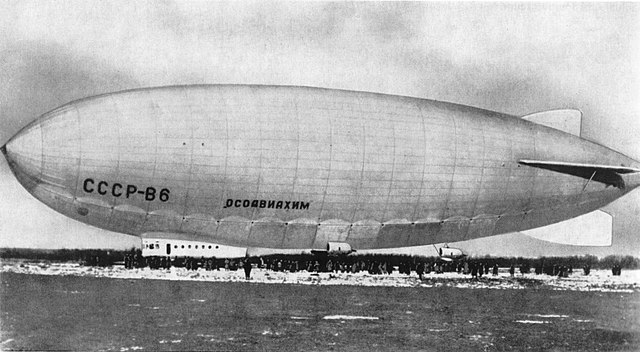
\includegraphics[width=\linewidth]{./chapter/aircraft/foto_of_airship.jpg}}
    }
	\caption{Airship.}
	\labfig{fig:airship_question_answers_aircraft_en}
\end{marginfigure}

Airship. 

Question from page~\pageref{question:aircraft_question_4}.

%%%%%%%%%%%%%%%%%%%%%%%%%%%%answer_5%%%%%%%%%%%%%%%%%%%%%%

\begin{exercise}%
\label{answer:aircraft_question_airship_2_en}
Which aircraft is shown in Fig. \ref{fig:airship_question_answers_aircraft_en}?

\end{exercise}

The aircraft shown in Fig. \ref{fig:airship_question_aircraft_en} is an airship. 
The answer to the question can also be obtained by running the following SPARQL-request (listing \ref{lst:aircraft_airship_photo_lst_en})

\begin{lstlisting}[ language=SPARQL, breaklines=true, 
                    caption={Airship images\\\hspace{\textwidth}
                        SPARQL query: \href{https://w.wiki/rg4}{w.wiki/rg4}
                        },
                    label=lst:aircraft_airship_photo_lst_en,
                    texcl 
                    ]
#defaultView:ImageGrid
SELECT ?airship ?airshipLabel ?image
WHERE
{
    ?airship wdt:P31 wd:Q133585. # instance of airship
  	?airship wdt:P18 ?image # image airship
    SERVICE wikibase:label { bd:serviceParam wikibase:language "en" }
}
\end{lstlisting}

Question from page~\pageref{question:aircraft_question_5}.

%%%%%%%%%%%%%%%%%%end_answers_aircraft%%%%%%%%%%%%%%%%%%%%%%%%%%%%%%


\section{From towns to cities with millions of inhabitants}
\labsec{answer-towns}

\begin{exercise}%
    \label{answer:cities_geographic_objects}
Which of the following cities were named after toponyms?
\begin{itemize}
\item \href{https://w.wiki/pzi}{Tolyatti}
\item \href{https://w.wiki/pzj}{Tula}
\item \href{https://w.wiki/pzk}{Chernyakhovsk}
\item \href{https://w.wiki/pzm}{Kurilsk}
\item \href{https://w.wiki/pzn}{Vologda}
\item \href{https://w.wiki/pzo}{Obninsk}
\end{itemize}
\end{exercise}

Tula, Kurilsk and Vologda were named after the following toponyms: Tulitsa river, \href{https://w.wiki/qqJ}{Kuril Islands}, \href{https://w.wiki/qqK}{Vologda river}. The answer to the question can also be obtained by running the following SPARQL query (Listing \ref{lst:cities_geographic_objects}). The \href{https://www.wikidata.org/wiki/Property:P138}{named after} property value shows which Wikidata object the city was named after.
    
\index{SPARQL!FILTER!Cities named after toponyms}
\begin{lstlisting}[ language=SPARQL, 
                    caption={Cities named after toponyms.\\\hspace{\textwidth}
                        SPARQL query: \href{https://w.wiki/otn}{w.wiki/otn}
                        },
                    label=lst:cities_geographic_objects,
                    texcl 
                    ]
SELECT ?city ?cityLabel ?namedAfterLabel ?whatIsItLabel WHERE {
	?city wdt:P31/wdt:P279* wd:Q7930989. # "city/town" subclasses
	?city wdt:P138 ?namedAfter. # with property "named after"
	?namedAfter wdt:P31 ?whatIsIt. # which is instance of
	FILTER(?city = wd:Q1341 || ?city = wd:Q2770 || ?city = wd:Q5655 
		|| ?city = wd:Q156046 || ?city = wd:Q1957 || ?city = wd:Q175651)
	SERVICE wikibase:label {bd:serviceParam wikibase:language "en"}
}
\end{lstlisting}%

See question on page~\pageref{question:cities_geographic_objects}.

\marginnote[-2.0cm]{
If it doesn't matter what certain type of city the Wikidata object belongs to, you can use a construction with subclasses, specifying the only class relative to which the search will be performed. This construction is discussed in more detail in the section  ``Wikidata completeness and disadvantages'' on page \pageref{section:countries_Wikidata_completeness_and_disadvantages}.
}

\begin{exercise}%
    \label{answer:cities_over_400_age}
Which of the following cities were founded more than 400 years ago: \href{https://w.wiki/pzt}{Moscow}, \href{https://w.wiki/pzu}{Sarov}, \href{https://w.wiki/pzx}{Kazan}, \href{https://w.wiki/pzy}{Astrakhan}, \href{https://w.wiki/pzz}{Samara}, \href{https://w.wiki/pz$}{Voronezh}?
\end{exercise}

Moscow (1147 year), Voronezh (1586), Samara (1586), Kazan (1005) and Astrakhan (1558) were founded more than 400 years ago. The answer to the question can also be obtained by running the following SPARQL query (Listing \ref{lst:cities_over_400_age}). The \href{https://www.wikidata.org/wiki/Property:P571}{inception} property value contains the date the city was founded.

\index{SPARQL!FILTER!Cities founded more than 400 years ago}
\index{SPARQL!BOUND!Cities founded more than 400 years ago}
\index{SPARQL!DATATYPE!Cities founded more than 400 years ago}
\index{SPARQL!BIND!Cities founded more than 400 years ago}
\begin{lstlisting}[ language=SPARQL, 
                    caption={Cities founded more than 400 years ago.\\\hspace{\textwidth}
                        SPARQL query: \href{https://w.wiki/oto}{w.wiki/oto}
                        },
                    label=lst:cities_over_400_age,
                    texcl 
                    ]
SELECT ?city ?cityLabel ?inceptionDate WHERE {
	?city wdt:P31/wdt:P279* wd:Q7930989. # "city/town" subclasses
	?city wdt:P17 wd:Q159. # belonging to Russia
	?city wdt:P571 ?inceptionDate. # with property "inception"
	FILTER(BOUND(?inceptionDate) && 
			DATATYPE(?inceptionDate) = xsd:dateTime).
	BIND(NOW() - ?inceptionDate AS ?distance).
	FILTER(0 <= ?distance && ?distance > 146000). # = 400 * 365
	FILTER(?city = wd:Q649 || ?city = wd:Q193522 || ?city = wd:Q900
		|| ?city = wd:Q3927 || ?city = wd:Q894 || ?city = wd:Q3426)
	SERVICE wikibase:label {bd:serviceParam wikibase:language "en"}
}
GROUP BY ?city ?cityLabel ?inceptionDate
\end{lstlisting}%

See question on page~\pageref{question:cities_over_400_age}.

\begin{exercise}%
    \label{answer:cities_flags}
Which city does the flag in \reffig{fig:flag_question_city} belong to?
\end{exercise}

The flag in \reffig{fig:flag_question_city} belongs to \href{https://w.wiki/qqN}{Karabulak}. The answer to the question can also be obtained by running the following SPARQL query (Listing \ref{lst:cities_flags}). The \href{https://www.wikidata.org/wiki/Property:P41}{flag image} property value contains the image of the city flag.

\index{SPARQL!FILTER!Cities flags}
\begin{lstlisting}[ language=SPARQL, 
                    caption={Cities flags.\\\hspace{\textwidth}
                        SPARQL query: \href{https://w.wiki/otp}{w.wiki/otp}
                        },
                    label=lst:cities_flags,
                    texcl 
                    ]
#defaultView:ImageGrid
SELECT ?city ?cityLabel ?flag ?countryLabel WHERE {
	?city wdt:P31/wdt:P279* wd:Q7930989. # "city/town" subclasses
	?city wdt:P17 ?country. # with property "country"
	?city wdt:P41 ?flag. # with property "flag"
	FILTER(?city = wd:Q144969) # for Karabulak only
	SERVICE wikibase:label {bd:serviceParam wikibase:language "en"}
}
\end{lstlisting}%

See question on page~\pageref{question:cities_flags}.

\section{Analysis of aspects of modern countries}
\labsec{answer-languages}
\begin{exercise}
\label{answer:population_density}
Identify the countries of Asia by flags and list them in ascending order of population density (fig. ~\ref{fig:flag_kor}, ~\ref{fig:flag_mongolia}, ~\ref{fig:flag_singapore}, ~\ref{fig:flag_israel}).
\end{exercise}

\begin{enumerate}
\item Mongolia (\num{1.96} people km\begin{math}^2\end{math}), (fig. ~\ref{fig:flag_mongolia});
\item Israel (\num{437.79} people km\begin{math}^2\end{math}), (fig. ~\ref{fig:flag_israel});
\item Korea (\num{513.14} people km\begin{math}^2\end{math}), (fig. ~\ref{fig:flag_kor});
\item Singapore (\num{8189.30} people km\begin{math}^2\end{math}), (fig. ~\ref{fig:flag_singapore}).
\end{enumerate}

The answer to the question can also be obtained by running the following SPARQL query (Listing \ref{lst:population_density}).

\begin{lstlisting}[ language=SPARQL, 
caption={\href{https://w.wiki/rcE}{
		Population density in Asia}\protect\footnotemark},
label=lst:population_density
]
SELECT ?country ?countryLabel ?flag ?area  ?population 
(?population / ?area as ?populationDensity)
{
	?country wdt:P31 wd:Q6256.       # country
	?country wdt:P30 wd:Q48 .        # on the continent of Asia
	?country wdt:P41 ?flag .         # has a flag (image)
	?country wdt:P2046 ?area .       # has an area
	?country wdt:P1082 ?population . # has a population
	
	SERVICE wikibase:label { bd:serviceParam wikibase:language "en" }
}
ORDER BY DESC(?populationDensity)
\end{lstlisting}

See question on page~\pageref{question:population_density}.
%%%%%%%%%%%%%%%%%%%%%%%%%%%%%%%%%%%%%%%%%%%%
\begin{exercise}
\label{answer:official_languages}
Which of these languages are official in \href{https://en.wikipedia.org/wiki/Russia}{Russia}?
\begin{itemize}
\item \href{https://en.wikipedia.org/wiki/Abaza_language}{Abaza};
\item \href{https://en.wikipedia.org/wiki/Moksha_language}{Moksha};
\item \href{https://en.wikipedia.org/wiki/Erzya_language}{Erzya};
\item \href{https://en.wikipedia.org/wiki/Belarusian_language}{Belarusian}.
\end{itemize}
\end{exercise}

The official languages of Russia are the Abaza, Moksha and Erzyan languages. The answer to the question can also be obtained by running the following SPARQL query (Listing \ref{lst:official_languages}).

\begin{lstlisting}[ language=SPARQL, 
caption={\href{https://w.wiki/rcF}{Official languages in Russia}\protect\footnotemark},
label=lst:official_languages
]
# Official language in Russia
SELECT ?lanquage ?lanquageLabel
WHERE
{
	?country wdt:P31 wd:Q6256 .# country
	?country wdt:P37 ?lanquage .
	FILTER(?country = wd:Q159) . 
	SERVICE wikibase:label { bd:serviceParam wikibase:language "en" }
}
\end{lstlisting}

See question on page~\pageref{question:official_language}.
%%%%%%%%%%%%%%%%%%%%%%%%%%%%%%%%%%%%%%%%%%%%
\begin{exercise}
\label{answer:administrative_territorial}

Latvia has 119, Thailand has 77, Denmark has 5, and Russia has 81. What are we talking about?
\begin{itemize}
\item Number of cities with a population of over one million;
\item Number of higher education institutions;
\item Number of administrative units;
\item Number of official languages.
\end{itemize}

\end{exercise}

We are talking about the number of administrative-territorial units in each country. The answer to the question can also be obtained by running the following SPARQL query (Listing \ref{lst:administrative_territorial}).

\begin{lstlisting}[ language=SPARQL, 
caption={\href{https://w.wiki/s86}{Number of administrative-territorial units in each country}\protect\footnotemark},
label=lst:administrative_territorial
]
#Contains administrative territorial entity in country
SELECT ?countryLabel  (count(*) as ?count)
WHERE
{
	?country wdt:P31 wd:Q6256.      # country
	?country wdt:P150 ?ATentity.    # contains administrative territorial entity 
	SERVICE wikibase:label { bd:serviceParam wikibase:language "en" }
}
GROUP BY (?countryLabel)
ORDER BY DESC(?count)
\end{lstlisting}

See question on page~\pageref{question:administrative_territorial}.

\section{Programming languages and its creators}
\labsec{answer-languages}
\begin{exercise}
    \label{answer:prog_lang_1}
Correlate a programming language and its developer.
	\begin{tabular}{ll}
		Developer & Language\\
		\hline
		J. Ichbiah & \href{https://www.wikidata.org/wiki/Q154755}{Ada}\\
		C. Moore & \href{https://www.wikidata.org/wiki/Q275472}{Forth}\\
		J. Armstrong & \href{https://www.wikidata.org/wiki/Q334879}{Erlang}\\
	\end{tabular}
\end{exercise}
    The Ada programming language was developed by Jean Ichbiah, Forth was developed by Charles H. Moore, and the creator of Erlang is believed to be Joe Armstrong. The answer to the question can also be obtained by running the following SPARQL query (listing \ref{lst:prog_lang_answer_1}). 
	\begin{lstlisting}[language=SPARQL, caption={{Programming languages developers}\protect\footnotemark}, label=lst:prog_lang_answer_1]
		SELECT ?item_label ?developer_label
		WHERE
		{
		 ?item wdt:P31 wd:Q9143
		 ; rdfs:label ?item_label. 
		 ?item wdt:P178 ?developer.
		 ?developer rdfs:label ?developer_label.
		 
		 FILTER (LANG(?item_label) = "en"). 
		 FILTER (LANG(?developer_label) = "en"). 
		}
		ORDER BY DESC (?item_label)
	\end{lstlisting}
SPARQL query: \href{https://w.wiki/kfZ}{https://w.wiki/kfZ}

Question from page~\pageref{question:prog_lang_1}.


\begin{exercise}
    \label{answer:prog_lang_2}
Which image is the programming language logo \href{https://www.wikidata.org/wiki/Q513238}{LOLCODE}:
    \begin{tabular}{c c c c}

\includegraphics[width=2cm]{./chapter/programming_language/task_2_logo_1.PNG} & 
\includegraphics[width=2cm]{./chapter/programming_language/task_2_logo_2.PNG} & 
\includegraphics[width=2cm]{./chapter/programming_language/task_2_logo_3.PNG} & 
\includegraphics[width=2cm]{./chapter/programming_language/task_2_logo_4.PNG}
	\end{tabular}
\end{exercise}
    The third picture is the logo of the LOLCODE programming language. The answer to the question can also be obtained by running the following SPARQL query (listing \ref{lst:prog_lang_answer_1}). 
	\begin{lstlisting}[language=SPARQL, caption={{Programmers languages logos}\protect\footnotemark}, label=lst:prog_lang_answer_1]
		#defaultView:ImageGrid
		SELECT ?item_label ?image
		WHERE
		{
		 ?item wdt:P31 wd:Q9143 # instances of programming language
		 ; rdfs:label ?item_label. 
		 ?item wdt:P154 ?image. # image
		 	
		 	FILTER (lang(?item_label) = "en")
}
	\end{lstlisting}
SPARQL query: \href{https://w.wiki/kfd}{https://w.wiki/kfd}

Question from page~\pageref{question:prog_lang_2}.


\begin{exercise}
    \label{answer:prog_lang_3}
Fill the gaps.

\href{https://www.wikidata.org/wiki/Q83303}{Fortran} ranks first in terms of the number of its dialects. Their number reaches about \underline{\hspace{1cm}}. In second place is \href{https://www.wikidata.org/wiki/Q132874}{Lisp}, it has \underline{\hspace{1cm}} dialects. The third place is shared by\href{https://www.wikidata.org/wiki/Q597330}{Standard ML} and \href{https://www.wikidata.org/wiki/Q633894}{Object Pascal} with \underline{\hspace{1cm}} dialects.
\end{exercise}
 It is believed that Fortran has 8 to 12 dialects, Lisp has 6 dialects, and Standard ML and Object Pascal have 3 dialects.
    
Question from page~\pageref{question:prog_lang_3}.

